\section{Adding ABS}
\label{sec:adding-abs}
Given the highly parametrized implementation, supporting an additional instruction set in a second version of the same processor is straightforward.
\subsection{Changes in the Control Unit}
As far as the decoding is concerned, the addition of the absolute value instruction amounts to adding a dedicated case in the combinational process describing the instruction decoder along with a specific ALU operation. The new ALU operation is just appended to the enumerated type that was already defined in the previous version. The new instruction is R-type and its opcode is 
\subsection{Changes on the Execution stage}
In order to best utilize the already available hardware, the addition of an ad-hoc unit was discarded. The adder path
is already used for nop-like operations, where the passed operand is simply summed to 0; being an adder/subtractor,
it also offers the possibility to invert the sign of one operand (specifically, operand 2), which is the only operation
needed in this case. For this reason, the only real changes happened at the controller level.

Given the generality of the description, accomodating for a new instruction did not require any change since its opcode
was simply added in the \texttt{t\_alu\_op} enumeration. In this specific case, the operand of interest is passed to
ALU's operand 2, but its inversion still needs to be conditional. This requires two additional signals to be sent to the
ALUController, called \texttt{operand1\_info} and \texttt{operand2\_info} of a newly described record type called
\texttt{t\_OperandInfo}.

Currently, an OperandInfo signal only keeps track of the sign of the operand, but it could also hold some additional
information\footnote{As discussed later, this connection between the operands paths and ALUController creates a longer
combinational path. It is best to keep the extracted information as simple as possible, only considering for instance
the operand's sign, its parity or a simple sticky bit.}. The controller, upon receiving the opcode corresponding to the
\texttt{ABS} operation, can simply check for operand2's sign and issue a subtraction only when the value is negative.

\begin{figure}[htbp]
    \center
	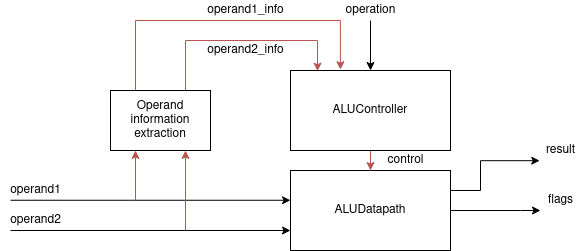
\includegraphics[width=0.8\textwidth]{./2-implementation/images/ALUWithABS.png}
	\caption{ALU with the new control paths needed for the implementation of ABS}
	\label{fig:alu-with-abs}
\end{figure}

The downside of this simple solution is a longer combinational path. Initially, the operand paths and the controls
path was separated: the controls were determined from the processor's Control Unit and the operands were
directly connected from their source to the datapath.\\
In this new scenario, operands also go through an information-extraction stage (which, in ABS case, does not add any
logic) and then go through ALUController as well, generating the control signals and finally arriving in the datapath.

If the extracted information is kept as simple as possible like in this case, where only the sign bit is sufficient to
perform the operation, the high level of controllability and customizability well justifies the introduced timing costs.
In the cases where a more complex operation is needed, instead, it is best to implement a custom unit to maintain
balance in the logical paths.
